\begin{frame}
\frametitle{The CMS detector}
\end{frame}
\begin{frame}\addtocounter{framenumber}{-1}
\frametitle{The CMS detector -- Silicon tracker (pixels)}
\begin{center}
detects charged particles going through

\vfill

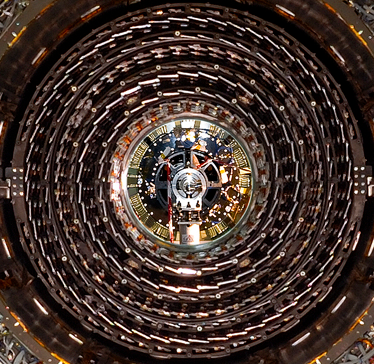
\includegraphics[width=\textwidth,height=0.75\textheight,keepaspectratio]{/home/torterotot/Documents/PhD-Thesis/tex/slides/LHC-CMS/CMS/CMS_zoomout_pictures/CMS_slice_photo_1-trk1.png}

\vfill

$\longleftarrow \SI{1}{\meter} \longrightarrow$
\end{center}
\end{frame}
\begin{frame}\addtocounter{framenumber}{-1}
\frametitle{The CMS detector -- Silicon tracker (strips)}
\begin{center}
detects charged particles going through

\vfill

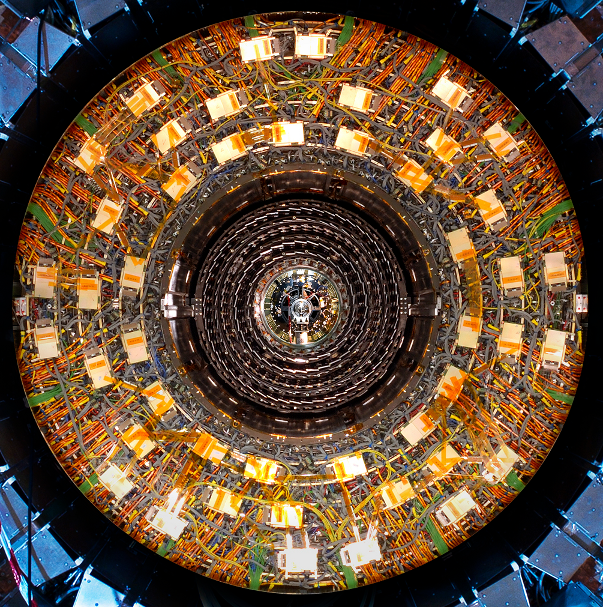
\includegraphics[width=\textwidth,height=0.75\textheight,keepaspectratio]{/home/torterotot/Documents/PhD-Thesis/tex/slides/LHC-CMS/CMS/CMS_zoomout_pictures/CMS_slice_photo_2-trk2.png}

\vfill

$\longleftarrow \SI{2}{\meter} \longrightarrow$
\end{center}
\end{frame}
\begin{frame}\addtocounter{framenumber}{-1}
\frametitle{The CMS detector -- Electromagnetic calorimeter (ECAL)}
\begin{center}
stops photons and electrons, measure their energies

\vfill

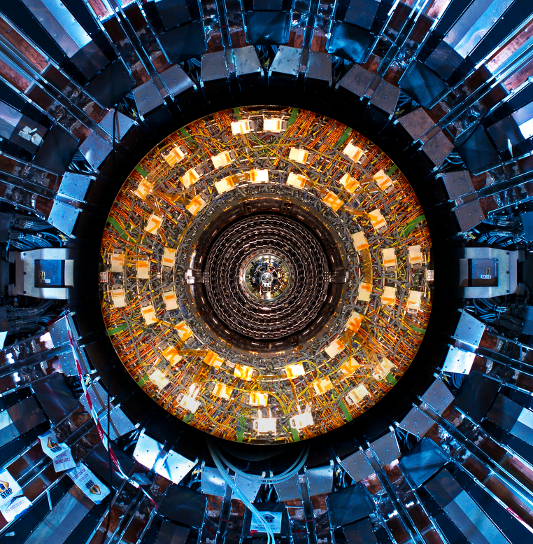
\includegraphics[width=\textwidth,height=0.75\textheight,keepaspectratio]{/home/torterotot/Documents/PhD-Thesis/tex/slides/LHC-CMS/CMS/CMS_zoomout_pictures/CMS_slice_photo_3-ECAL.png}

\vfill

$\longleftarrow \SI{3}{\meter} \longrightarrow$
\end{center}
\end{frame}
\begin{frame}\addtocounter{framenumber}{-1}
\frametitle{The CMS detector -- Hadron calorimeter (HCAL)}
\begin{center}
stops hadrons (protons, neutrons, ...), measure their energies

\vfill

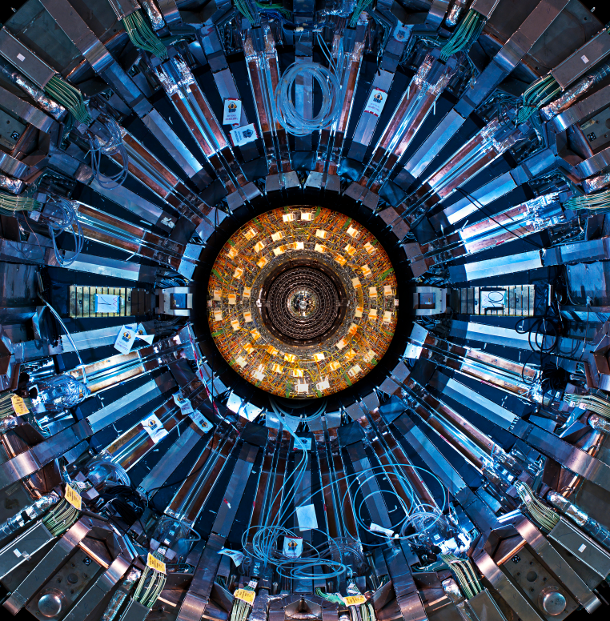
\includegraphics[width=\textwidth,height=0.75\textheight,keepaspectratio]{/home/torterotot/Documents/PhD-Thesis/tex/slides/LHC-CMS/CMS/CMS_zoomout_pictures/CMS_slice_photo_4-HCAL.png}

\vfill

$\longleftarrow \SI{5}{\meter} \longrightarrow$
\end{center}
\end{frame}
\begin{frame}\addtocounter{framenumber}{-1}
\frametitle{The CMS detector -- Superconducting solenoid}
\begin{center}
creates a \SI{4}{\tesla} magnetic field which bends charged particles trajectories

\vfill

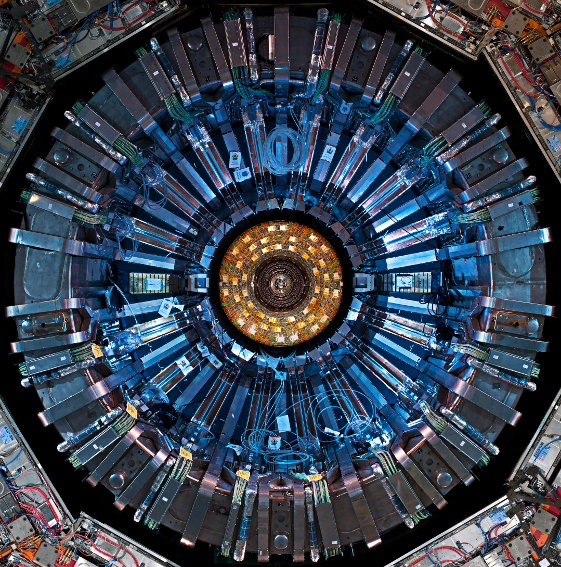
\includegraphics[width=\textwidth,height=0.75\textheight,keepaspectratio]{/home/torterotot/Documents/PhD-Thesis/tex/slides/LHC-CMS/CMS/CMS_zoomout_pictures/CMS_slice_photo_5-solenoid.png}

\vfill

$\longleftarrow \SI{7}{\meter} \longrightarrow$
\end{center}
\end{frame}
\begin{frame}\addtocounter{framenumber}{-1}
\frametitle{The CMS detector -- Muon system}
\begin{center}
detects muons going through

\vfill

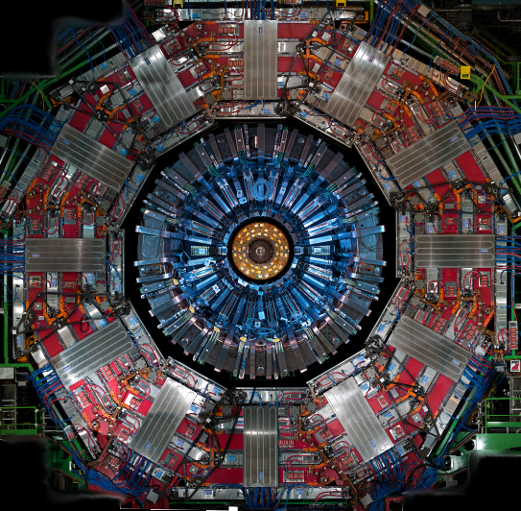
\includegraphics[width=\textwidth,height=0.75\textheight,keepaspectratio]{/home/torterotot/Documents/PhD-Thesis/tex/slides/LHC-CMS/CMS/CMS_zoomout_pictures/CMS_slice_photo_6-muons.png}

\vfill

$\longleftarrow \SI{15}{\meter} \longrightarrow$
\end{center}
\end{frame}